\chapter{Beschreibung des Programmablaufs}
Über einen konfigurierbaren Crawler können HTML-Inhalte von Webseiten bis zu einer bestimmten Tiefe
aus dem Netz in ein Archiv geladen werden. Da dies parallelisiert erfolgen soll,
müssen die Daten nach dem Herunterladen von temporären Verzeichnissen in das gemeinsame
Archivverzeichnis synchronisiert werden. Der aus der URL extrahierte Pfad der HTML-Dateien wird
dabei auf das Archiv abgebildet, wobei jede HTML-Datei in einen eigenen Archivordner verschoben wird. \\
Beim Crawlvorgang werden zusätzlich Metadaten der HTML-Seiten erstellt. 
Diese werden in einer Datenbank und als XML-Datei im jeweiligen HTML-Ordner gespeichert.
Die Datenbank soll dabei wieder aus den XML-Daten rekonstruierbar sein. \\
Außerdem sollen Filter eingehängt werden können, die bereits in den TMP-Ordnern ungültige Dateien löschen.
Über eine Java-Schnittstelle kann anschließend wieder auf die Daten zugegriffen werden.
Dabei sollen neben dem Auslesen von vorhandenen Dateien auch neue Dateien den Archivordnern hinzugefügt werden können.
Ebenso sollen die oben genannten XML-Daten um neue Nodes erweiterbar sein.
Zu Vorführzwecken wird ein Testanalysetool erstellt, welches die bereitgestellte Schnittstelle testet.

\chapter{Datenmodell der Metadaten}
Für vereinfachte Such- und Sortieraufgaben wird bereits ein vereinfachtes Datenmodell festgelegt, welches
später auf Datenbank und XML-Daten umgesetzt werden soll und zentrale Metadaten über HTML-Seiten erfassen soll.
Die XML-Dateien sollen grundsätzlich um neue Tags/Nodes erweitert werden können, die Datenbank darf davon aber nicht betroffen sein.
\begin{table}[h]
\centering
\begin{tabular}{|l|l|}	
	\hline
	Name & Datentyp \\
	\hline
	URL & String \\
	Titel des Dokuments & String \\ %?? kopiert aus Anforderung
	Dateipfad des Archivordners im Archiv & String \\
	Datum der letzten Änderung & TimeStamp oder Integer \\
	Commit Tag der Versionsverwaltung & String \\
	\hline
\end{tabular}
\caption{Metadaten}
\end{table}

\chapter{Anforderungen}
Im folgenden sind die Anforderungen an die Software spezifiziert. Soweit möglich wurden
die Anforderungen schon in einzelne Komponenten und Module gegliedert. Eine grobe Übersicht gibt auch Diagramm \ref{spec:dia:moduls}
\section{Crawlermodul}
Dieses Modul soll als eigenständiger Prozess laufen und in regelmäßigen Abständen Crawlvorgänge starten
und die Daten in das Archiv schreiben.

\subsection{Steuerung} \label{spec:req:crawler:control}
	\subsubsection{Config-Datei} \label{spec:req:crawler:control:config} 
		Die Steuerung des bzw. der Crawler erfolgt über eine Config-Datei.
		Darin werden bereits Default- und Fallbackwerte festgelegt  
		Es können folgende Parameter eingestellt werden:
		\begin{enumerate}
			\item Tiefe bis zu der Links gefolgt werden soll
			\item Zeitintervalle der Crawlvorgänge
			\item maximale Anzahl der gleichzeitig gestarteten Crawlerinstanzen
			\item Filtereinstellungen
		\end{enumerate}
	\subsubsection{Kommandozeileninterface} \label{spec:req:crawler:control:cmd} 
		Optional können beim Start mittels Kommandozeile zusätzliche Parameter übergeben werden:
		\begin{itemize}
			\item Damit lassen sich Werte aus der Config-Datei überschreiben.
			\item Es kann man eine Liste von Domains übergeben werden, die als Startpunkte für die Crawler verwendet werden sollen.
				Wobei mindestens ein Element obligatorisch ist.
			\item Es kann ein Datenbank-Recovery erzwungen werden. siehe \label{db:recovery}
		\end{itemize}
\subsection{Ausführung des Crawlvorgangs}
	Die Folgenden Teilvorgänge sind so ausgelegt, dass sie parallelisiert abgearbeitet werden können.
	\subsubsection{Instanziierung} \label{spec:req:crawler:instance}
		Pro Domain wird eine Crawlerinstanz gestartet bis die Obergrenze an Instanzen erreicht wird.
		Für die Crawlerinstanzen wird ein externes Tool verwendet (z.B. wget).
		Jede gestartete Instanz kopiert den Inhalt der Seite in je ein temporäres Verzeichnis.
		Dabei wird die online vorhandene URL-Pfadstruktur der HTML-Dateien auf das Dateisystem abgebildet.
		Je Domain wird dadurch ein Hauptverzeichnis erzeugt.
	\subsubsection{Bereinigung und Normalisierung} \label{spec:req:crawler:normalize}
		Nun werden die temp-Ordner bereinigt (z.B. leere Ordner entfernt)
		und die HTML-Dateien in ein Archiv-Ordner gleichen Namens (inklusive Dateiendung) kopiert.
	\subsubsection{Filterung} \label{spec:req:crawler:filter}
		Die Daten werden in diesem Teilvorgang von Filtern überprüft und ggf. gleich aussortiert.
	\subsubsection{Extraktion der Metadaten}\label{spec:req:crawler:extraction}
		In diesem Teilvorgang werden die Metadateien im XML-Format extrahiert und jeweils als Datei im zugehörigen Archivordner gespeichert.
	\subsubsection{Synchronisation}\label{spec:req:crawler:sync}
		Zuletzt werden die so vorbereiteten temporären Ordner in das vorhandene Archiv synchronisiert (z.B. mit rsync). 
		Dabei wird jeder Domainordner über ein Dateimutex gesperrt, um gleichzeitiges Schreiben zu verhindern. 
		Veraltete Archivordner werden dabei komplett überschrieben (können aber ggf. durch die Versionierung wieder hergestellt werden),
		sodass auch veraltete Analysedaten gelöscht werden.\\
		Zum Abschluss werden die Änderungen den Versionsverwaltungen der Domainordner mit einem Commit bestätigt.
	\subsubsection{Datenbankaktualisierung}
		Während oder nach dem Synchronisationsvorgang wird ein Batch von SQL-Statements für die neuen oder geänderten Daten
		zur Aktualisierung der Datenbank erstellt.
\subsection{Filter}
	Filter können über die Konfiguration beim Starten bekannt gemacht werden und werden als Module/Plugins hinzugefügt.
	Während des Teilvorgangs \ref{spec:req:crawler:filter} erhalten diese eine HTML-Datei und geben nach Prüfung einen Wahrheitswert zurück
	ob die übergebene HTML-Datei behalten werden soll.
	\subsubsection{Testfilter: Englische Sprache}
		Als Testfilter wird ein Filter implementiert, der nichtenglische Seiten aussortiert.


\section{Archiv} \label{spec:req:archive}
\subsection{Aufteilung:}\label{spec:req:archive:dist}
	Das Verzeichnis ist in einzelne Domainordner getrennt. 
\subsection{Versionierung:}\label{spec:req:archive:vers}
	Jeder Domainordner wird über ein Versionsverwaltung (z.B. git) versioniert. 
	Damit ist das Wiederherstellen älterer Versionen grundsätzlich möglich,
	wobei diese aber manuell über die git-Schnittstellen abgerufen werden müssen.
	Änderungen an Dateien müssen immer mit einem Commit bestätigt werden.
\subsection{Synchronisation}\label{spec:req:archive:sync}
	Bei Schreibvorgängen muss ähnlich wie unter \ref{spec:req:crawler:sync} beschrieben, 
	die Daten gegen konkurrierende Dateizugriffe gesichert werden.
	Dabei wird immer der ganze Domainordner gesperrt.
\subsection{Dateisystem:} \label{spec:req:archive:fs}
	Beim darunterliegenden Dateisystem wird von einem vorhandenen Unix-FS ausgegangen.
\subsection{Komprimierung:} \label{spec:req:archive:comp}
	Eine explizite Dateikomprimierung wird erstmal nicht vorgesehen, ist aber zum Teil schon durch die Versionierung gegeben.
	In der Regel werden alte Revisionen gepackt.

\section{Programmierschnittstelle - Java-Client/Server}\label{spec:req:jcs}
	Diese Schnittstelle soll die Anbindung der Analysemethoden ermöglichen und macht gleichzeitig einen Zugriff über das Netzwerk möglich.
\subsection{Schnittstelle - Client}\label{spec:req:jcs:client}
	\subsubsection{Datenbankabfragen} \label{spec:req:jcs:client:dbquery}
		Über diesen Client können vorbereitete SQL-Statements an einen Java-Server geschickt werden. 
		Die SQL-Abfrage wird soweit vorbereitet, dass nur noch ein SQL-Bedingungsausdruck für die WHERE-Klausel angegeben werden muss.
		Optional soll auch eine ORDER-BY-Klausel im selben Stil angegeben werden können. 
		Als return-Wert wird eine Liste von Metadatenobjekten zurückgegeben.
	\subsubsection{Dateiabfrage} \label{spec:req:jcs:client:fsquery}
		Mittels der Metadatenobjekte kann man sich über eine gesonderte Anfrage die vorhandenen Archivordner aus dem Archiv nachladen.
\subsection{Metadatenklasse} \label{spec:req:jcs:meta}
	Die Metadatenklasse dient nicht nur als Schlüssel zur Dateianfrage ans Archiv sondern auch zur Erweiterung und Auslesen der XML-Daten.
	\subsubsection{Auslesen von Zusätzlichen Tags} \label{spec:req:jcs:meta:select}
		Durch Übergabe eines Tagnamens an eine get-Methode wird ein passender XML-Node herausgesucht wird.
	\subsubsection{Erweiterung	der XML-Dateien} \label{spec:req:jcs:meta:insert}
		Mittels einer set-Methode, die Namen und Inhalt des Tags als Parameter erhält, können neue Tags hinzugefügt werden.
		Die XML-Datei muss daraufhin automatisch gesichert werden.
\subsection{Server} \label{spec:req:jcs:server}
	Im Hintergrund nimmt ein Java-Server die Nachrichten der Clients entgegen
	und führt die o.g. Funktionen aus und gibt die Ergebnisse oder Fehlermeldungen an den Client zurück.
	Datei- und Datenbankfunktionen können evtl. mit dem Crawlermodul geteilt werden.

\section{Test Analysetool}
	Zur Demonstrations- und Testzwecken der Java-Clientschnittstelle wird ein Analysetool erstellt, welches bestimmte Wörter zählt
	und das Ergebnis im Archiv als Datei sowie im XML als zusätzliches Tag speichert.

\section{Datenbank} \label{spec:req:db}
	Die Datenbank dient zur Speicherung der grundlegenden Metadaten und soll schnelle Suchanfragen ermöglichen.
\subsection{Zugriff}
	Der Zugriff erfolgt grundsätzlich nur über die bereitgestellten Schnittstellen.
\subsection{Aktualisierung} \label{spec:req:db:update}
	Die Datenbank muss beim Fertigstellen des Crawlvorgangs auf den neuesten Stand gebracht werden.
\subsection{Wiederherstellung} \label{spec:req:db:recovery}
	Sollte die Datenbank beschädigt oder geändert werden, dann soll diese wieder aus den
	XML-Metadaten rekonstruiert werden können.
	Aus diesem Grund wird erstmal von einer sqlite-Datenbank ausgegangen, 
	da diese relativ einfach als Datei erstellt und wieder gelöscht werden kann.

\section{XML-Dateien} \label{spec:req:xml}
	Für die Validierung der XML-Daten muss eine XML-Schema ausgearbeitet werden.
	Besonderes Augenmerk ist hierbei auf die Erweiterbarkeit zu legen.

\section{Entwicklungsumgebung} \label{spec:req:devenv}
\subsection{Programmiersprachen}
	Es werden die Sprachen Python und Java benutzt.
	\subsubsection{Python}
		Python in der Version 2 (2.7) wird für die systemnahen Teile verwendet, wie das gesamte Crawlermodul, 
		der Zugriff auf das Dateisystem (Archiv) und die notwendige Ordnersynchronisation, 
		da hier bereits leistungsfähige Libraries für den Zugriff auf das Dateisystem und die Versionsverwaltung vorhanden sind.
	\subsubsection{Java}
		Die Client-Server Architektur der oben genannten Programmierschnittstelle werden mit Java 1.7 umgesetzt.
		Hierzu ist Java besonders geeignet und es ist gewährleistet, eine an der Hochschule Hof allgemein verständliche
		Schnittstelle zu schaffen.
\subsection{Dokumentation}
	Die Dokumentation wird in Latex als ein fortlaufendes Gesamtdokument erstellt, welches je nach Phase um weitere Teile erweitert wird.
\subsection{Teamsynchronisation}
	Dokumente und Quellcode werden über ein gemeinsames Repository bei github.com synchronisiert.
\subsection{Sprache}	
	Die Sprache der Dokumentation ist Deutsch wobei natürlich geläufige Fremdwörter enthalten sind. Quellcode, Kommentare und daraus abgeleitete APIs (z.B. Javadoc) sind in Englisch zu verfassen.

\newpage 
% Diagramm

\begin{figure}
	\centering
	\label{spec:dia:moduls}
	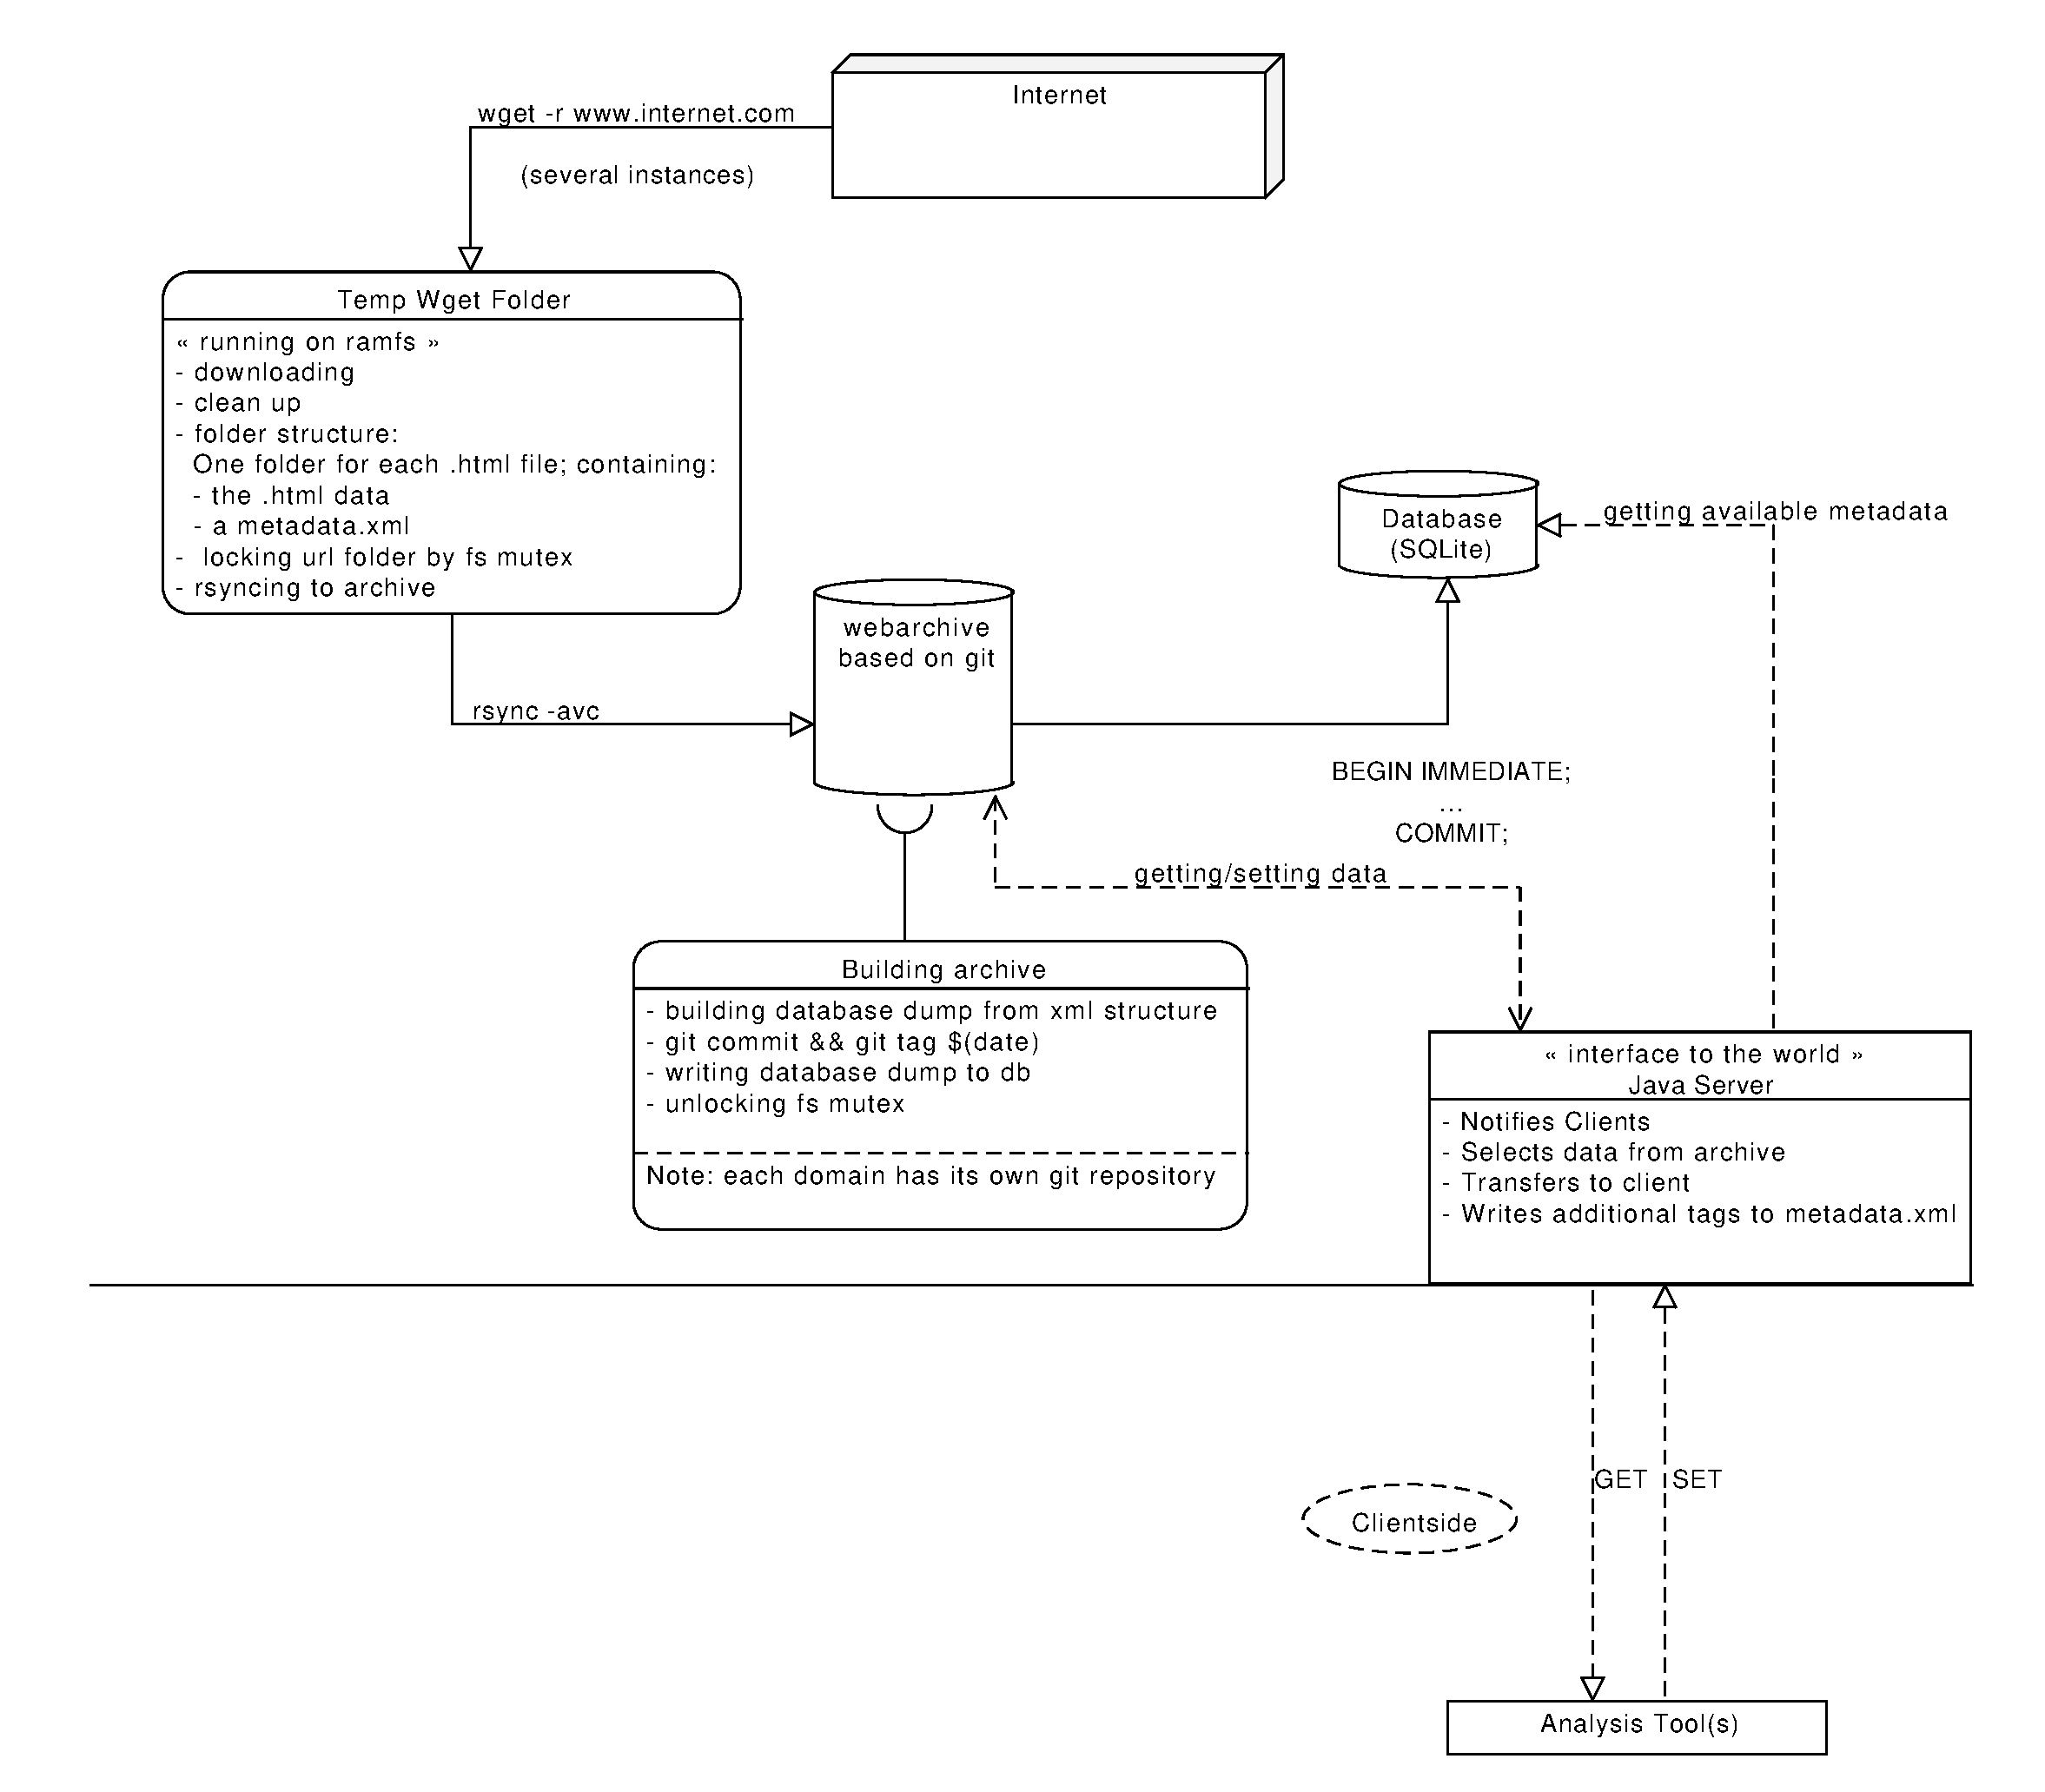
\includegraphics[width=\textwidth]{spezi/webarchiv_design.pdf}
	\caption{Diagramm: Grundlegendes Design}
\end{figure}
 
